\documentclass[12pt]{iopart}

\usepackage{iopams}
\usepackage{graphicx}  
\usepackage{url}

% some definitions 
\def\be{\begin{equation}}
\def\ee{\end{equation}}
%
\def\bea{\begin{eqnarray}}
\def\eea{\end{eqnarray}}
%

\begin{document}

%\title[The second round of MLDCs]{An overview of the second round of the Mock LISA Data Challenges}
\title[The second round of Mock LISA Data Challenges]{An overview of the second round of the Mock LISA Data Challenges}

\author{K A Arnaud$^1$,
S Babak$^2$,
J Baker$^1$,
M J Benacquista$^3$
N J Cornish$^4$,
C Cutler$^{5}$,
L S Finn$^{6}$,
S L Larson$^{7}$,
E K Porter$^{2,4}$,
B S Sathyaprakash$^{8}$,
M Vallisneri$^{5}$,
A Vecchio$^{9,10}$,
J-Y Vinet$^{11}$\\
\centerline{(The Mock LISA Data Challenge Task Force)}
}

\address{$^1$ Gravitational Astrophysics Laboratory, NASA Goddard Space Flight Center, 8800 Greenbelt Rd, Greenbelt, MD 20771, US}
\address{$^2$ Max-Planck-Institut f\"{u}r Gravitationsphysik (Albert-Einstein-Institut), Am M\"{u}hlenberg 1, D-14476 Golm bei Potsdam, Germany}
\address{$^3$ Center for Gravitational Wave Astronomy, University of Texas at Brownsville, Brownsville, TX 78520, US}
\address{$^4$ Dept.\ of Phys., Montana State University, Bozeman, MT 59717, US}
\address{$^{5}$ Jet Propulsion Laboratory, California Institute of Technology, Pasadena, CA 91109, US}
\address{$^{6}$ Center for Gravitational Wave Physics, The Pennsylvania State University, University Park, PA 16802, US}
\address{$^{7}$ Dept.\ of Phys., Weber State University, 2508 University of Circle, Ogden, UT 84408, US}
\address{$^{8}$ Dept.\ of Phys.\ and Astron., Cardiff University, 5, The Parade, Cardiff, CF24 3YB, UK}
\address{$^{9}$ School of Phys.\ and Astron., University of Birmingham, Edgbaston, Birmingham B152TT, UK}
\address{$^{10}$ Dept.\ of Phys.\ and Astron., Northwestern University, Evanston, IL 60208, US}
\address{$^{11}$ Department ARTEMIS, Observatoire de la C\^{o}te d'Azur, BP 429, 06304 Nice, France}
\ead{lisatools-mldc@gravity.psu.edu}
\begin{abstract}
The Mock Data Challenges (MLDCs) have the dual purpose of fostering the development of LISA data analysis tools and capabilities, and demonstrating the technical readiness already achieved by the gravitational-wave community in distilling a rich science payoff from the LISA data. The first round of MLDCs has just been completed and the second round data sets have been released. The round two data sets contain radiation from an entire Galactic population of stellar-mass binary systems, massive black hole binaries and extreme-mass-ratio inspirals. These data sets are designed to capture much of the complexity that is expected in the actual LISA data, and should provide a fairly realistic setting to test advanced data analysis techniques, and in particular the aspect of global data analysis. Here we describe the second round of MLDCs and provide details about its implementation.

\end{abstract}

%Uncomment for PACS numbers title message
%\pacs{00.00, 20.00, 42.10}
% Keywords required only for MST, PB, PMB, PM, JOA, JOB? 
%\vspace{2pc}
%\noindent{\it Keywords}: Article preparation, IOP journals
% Uncomment for Submitted to journal title message
%\submitto{\JPA}
% Comment out if separate title page not required
%\maketitle

\section{Introduction}
\label{s:intro}

The Laser Interferometer Space Antenna (LISA) is a spaceborne gravitational-wave (GW) laser-interferometer for the observation of the low-frequency  ($\approx$ 0.1 mHz-- 1 Hz) GW sky (see \cite{ScienceCase,lisappa} and Danzmann's contribution in this volume). LISA is an all-sky monitor with the capability of observing a variety of compact-object binary systems, with masses ranging from a fraction to millions of solar masses. Moreover, LISA could discover GWs from entirely new classes of sources, such as exotic compact objects and relics from the early universe (see \cite{ScienceCase,CT2002} and references therein).

The vast majority of LISA sources are visible for months to years in the instrument observational window. Strong GW foregrounds generated by abundant populations of Galactic and extra-Galactic white-dwarf binary systems, and possibly by solar-mass compact objects captured by massive black holes in galactic nuclei, will appear above the instrumental noise at frequencies below a few mHz. Some signals, such as the extreme-mass-ratio inspirals (EMRIs) are instantaneously weak and characterized by complex amplitude and phase evolution controlled by over a dozen parameters. Indeed, there is no established expertise for this kind of data, although much relevant experience has already been gained in the analysis of GW data collected by ground-based detectors. In ground-based observations GWs are rare and weak, whereas in the low-frequency band they are numerous and (a fair fraction of them) yield high signal-to-noise ratios (SNR). An important step in preparation for the mission is to tackle these new analysis problems early, in order to develop the tools and methods necessary for the maximum science exploitation of such a revolutionary data set.

The LISA International Science Team (LIST) has embarked on a programme to foster the development of data analysis tools and capabilities for LISA, and to evaluate the technical readiness of these tools. This programme goes under the name of Mock LISA Data Challenges (MLDCs). The MLDC Task Force%
\footnote{Full details regarding the Task Force activities, as well as links to relevant resources, are available on the Task Force wiki~\cite{MLDCwiki}.}
% 
has been charged by the LIST to formulate challenge problems, develop standard models of the LISA mission and gravitational wave sources, provide computing tools (e.g., LISA response simulators, and source waveform generators), establish criteria for the evaluation of the responses to the challenges, and provide any technical support necessary to the challenge participants. These challenges are meant to be blind tests, but not really contests; the greatest scientific benefit stemming from them will come from the quantitative comparison of results, analysis methods, and implementations.

The first round of MLDCs~\cite{MLDCLISA06a,MLDCLISA06b} has just been completed. Details on the data sets, techniques developed for the analyses, and results are provided in the companion article in this volume~\cite{MLDC1-gwdaw}, and references therein. In this short paper we describe the second round of MLDCs, which has just been released~\cite{MLDCweb}. The second-round data sets represent a very significant increase in complexity with respect to those distributed in Challenge 1. More importantly, they contain the full set of key signals that are expected to make up the LISA data set, and therefore provide a reasonably realistic testbed for different data analysis approaches. The instrument response, instrument noise, and waveform models adopted so far in the MLDCs employ various simplifications: much work is therefore required beyond the completion of Challenge 2 to develop the analysis tools necessary for the mission, and future round of MLDCs will address progressively more realistic analysis scenarios and introduce more general gravitational waveforms. The details of the schedule of MLDCs from Challenge 3 onwards have not been decided yet, but we expect to release the third round of MLDCs in Summer 2007.

\section{Mock LISA Data Challenges: Second round}
\label{s:MLDC2}

The first round of MLDCs contained single source data sets, or data sets with several ($\approx 20$) signals well separated in parameter space; an exception were two data sets containing $\approx 50$ signals from Galactic binaries, concentrated in frequency bands of width 30 $\mu$Hz and 3 $\mu$Hz. Challenge 1 focused on only two signal classes: Galactic stellar mass binaries and massive-black-hole (MBH) binary inspirals. The key goal of this first round of challenges was the development and validation of source specific data analysis techniques for the minimum science requirement signals. Challenge 2 has a much more realistic flavour: it includes millions of Galactic binaries,
as we expect in reality, in addition to multiple massive-black hole binaries and EMRIs. Thus, this round of challenges will require analysts to tackle \emph{global analysis} in the presence of the most challenging signals that we expect to observe with LISA. 

Challenge 2 includes five single-source data sets (Challenge 1.3.1)%
\footnote{These data sets are still identified by 1.X because training data sets were distributed with Challenge 1; blind data sets are however released only now. For consistency with previous documents, we maintain the original nomenclature.},
% 
dedicated specifically to EMRIs, and two multi-source data sets (Challenge 2.1 and 2.2). All the data sets are all $\approx 2$ years long---they contain $2^{22}$ data points sampled at a cadence of 15 sec. More specifically,
the data sets are as follows: 
\begin{itemize}
\item \emph{Challenge 1.3.1} consists of five data sets, each of which contains radiation from a single EMRI with SNR approximately in the range 40--110;
\item \emph{Challenge 2.1} contains radiation from (i) a whole population of Galactic binary systems (about 26 million sources), including (ii) 20 ``verification binaries'';
\item \emph{Challenge 2.2} contains radiation from (i) a whole population of Galactic binary systems (about 26 million sources), including (ii) 20 ``verification binaries''; (iii) an \emph{unknown} number (between 4 and 6) of MBH binaries with a range of SNRs (between $\approx 2000$ and $\approx 10$) and coalescence times; and (iv) 5 EMRIs, with SNRs in the range $\approx 30-100$.
\end{itemize}
Details about the range of the source parameters included in the data sets are given in Table~\ref{t:MLDC2}. An example of a typical Challenge 2.2 data set is shown in Figure~\ref{f:C2.2}. As data sets 2.1 and 2.2 contain millions of Galactic binary sources, the Task Force has identified 4 frequency bands on which analysis should concentrate first, and over which the evaluation of the results will be carried out in much more depth: these windows  are 0.2985 mHz $\le f \le$ 0.3015 mHz, 0.9985 mHz $\le f \le$ 1.0015 mHz, 2.9985 mHz $\le f \le$ 3.0015 mHz, and 5.9985 mHz $\le f \le$ 6.0015 mHz.  

%------------------------------    BIG TABLE   -------------------------------
\begin{table}
\begin{tabular}{llll}
\hline
Challenge & Sources & Parameters \\
\hline
\multicolumn{2}{l}{1.3.1} & \\
&Extreme-mass-ratio inspirals & $\mu/M_\odot \in U[9.5,10.5]$, $S/M^2 \in U[0.5, 0.7]$ \\
&                                             & time at plunge $\in  U[2^{21},2^{22}] \times 15$ sec \\
&                                             & eccentricity at plunge $\in U[0.15, 0.25]$ \\
1.3.1a &\multicolumn{1}{r}{\ldots one source with}          & $M / 10^7 M_\odot \in U[0.95,1.05]$ \\
1.3.1b &\multicolumn{1}{r}{\ldots one source with}         & $M / 10^6 M_\odot \in U[4.75,5.25]$ \\
1.3.1c &\multicolumn{1}{r}{\ldots one source with}         & $M / 10^6 M_\odot \in U[4.75,5.25]$ \\
1.3.1d &\multicolumn{1}{r}{\ldots one source with}         & $M / 10^6 M_\odot \in U[0.95,1.05]$ \\
1.3.1e &\multicolumn{1}{r}{\ldots one source with}         & $M / 10^6 M_\odot \in U[0.95,1.05]$ \\
\hline

2.1 & & \\
&Galactic binaries & drawn from a population (see Sec~\ref{ss:galaxy})\\
&\multicolumn{1}{r}{about $3\times 10^7$ sources} & \\
&Verification binaries & see parameters in the XML file posted on~\cite{MLDCweb}\\
&\multicolumn{1}{r}{20 sources} \\
\hline
2.2 & & \\
&Galactic binaries & drawn from a population (see Sec~\ref{ss:galaxy})\\
&\multicolumn{1}{r}{about $3\times 10^7$ sources} \\
&Verification binaries & see parameters in the XML file posted on~\cite{MLDCweb} \\
&\multicolumn{1}{r}{20 sources} & \\
&Massive-black-hole binary & $m_1/10^6\,M_\odot \in U[1,5]$, $m_2/m_1 \in U[1,4]$ \\
&\multicolumn{1}{r}{\ldots source n.1} &  $(t_\mathrm{in} - t_c) \in U[60,90]$ days \\
&\multicolumn{1}{r}{\ldots source n.2} &  $(t_\mathrm{in} - t_c) \in U[750,780]$ days \\
&\ldots and 2 out of 4 sources chosen from \ldots & \\
&\multicolumn{1}{r}{\ldots source n.3} & $(t_\mathrm{in} - t_c) \in U[180,720]$ days \\
&\multicolumn{1}{r}{\ldots source n.4} &  $(t_\mathrm{in} - t_c) \in U[180,720]$ days\\
&\multicolumn{1}{r}{\ldots source n.5} &  $(t_\mathrm{in} - t_c) \in U[495,585]$ days\\
&\multicolumn{1}{r}{\ldots source n.6} &  $(t_\mathrm{in} - t_c) \in U[801,840]$ days\\
&Extreme-mass-ratio inspirals & $\mu/M_\odot \in U[9.5,10.5]$, $S/M^2 \in U[0.5, 0.7]$ \\
&                                             & time at plunge $\in  U[2^{21},2^{22}] \times 15$ sec \\
&                                             & eccentricity at plunge $\in U[0.15, 0.25]$ \\
&\multicolumn{1}{r}{\ldots one source with}          & $M / 10^7 M_\odot \in U[0.95,1.05]$ \\
&\multicolumn{1}{r}{\ldots two sources with}         & $M / 10^6 M_\odot \in U[4.75,5.25]$ \\
&\multicolumn{1}{r}{\ldots two sources with}         & $M / 10^6 M_\odot \in U[0.95,1.05]$ \\
\hline
\end{tabular}
\caption{Summary of data sets and signal parameter ranges in the second round of MLDCs. All angular parameters are drawn randomly from a uniform distribution over the whole relevant range. The distance of the source is again drawn randomly, with the constraint to approximately provide the SNR at which the signal was designed to appear. In this Table, $t_\mathrm{in}$ corresponds to the beginning of the observation (i.e., the time stamp of the first data sample); $U[.]$ stands for uniform distribution within the given range. Notice that the single-source data sets in Challenge 1.3 drawn from the same parameter range (b-c and d-e) differ mainly in SNR, as well as the actual EMRI parameters. The same apply to the multiple source data set 2.2.}
\label{t:MLDC2}
\end{table}
%------------------------------    END TABLE   -------------------------------

%------------------------------    FIGURE   -------------------------------
\begin{figure}[htb]
\input{epsf}
\centerline{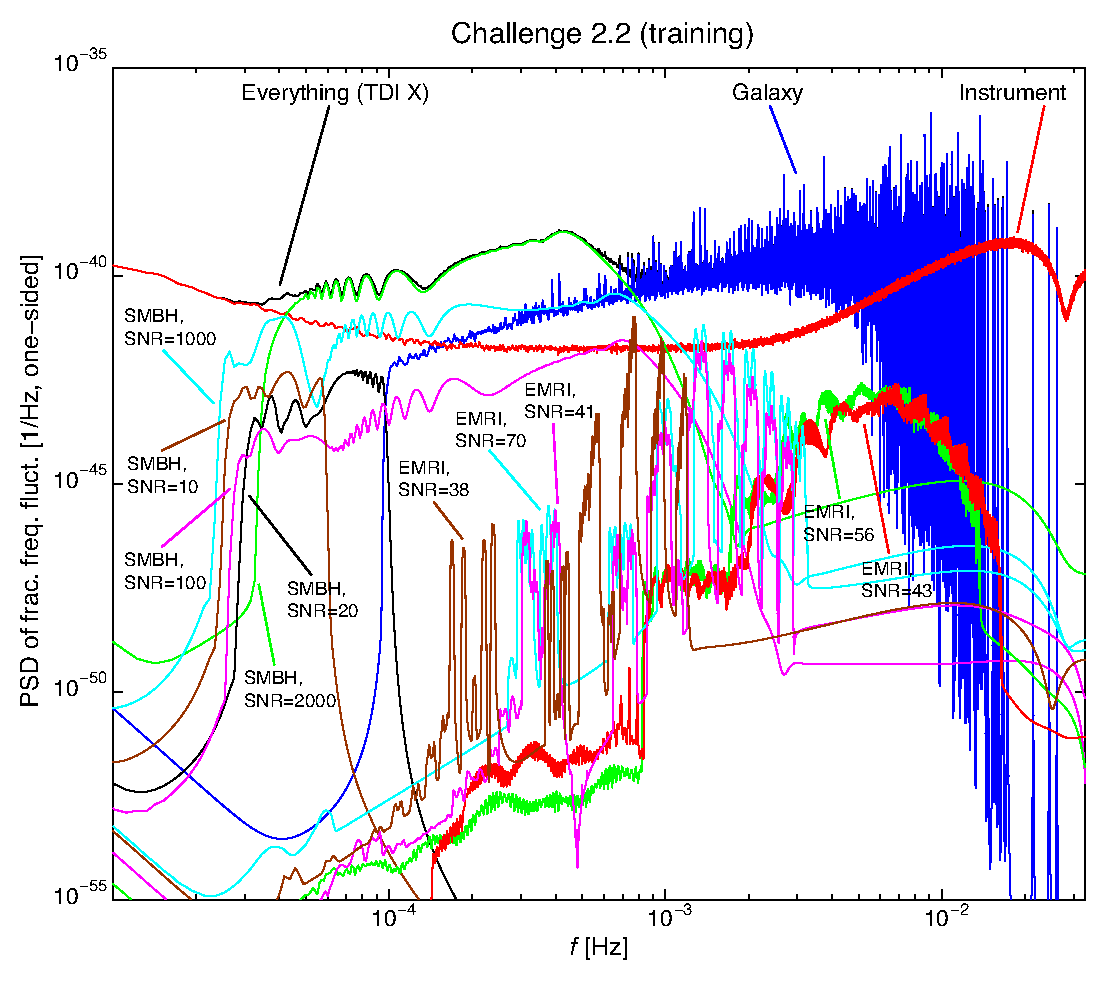
\includegraphics[height=8cm]{challenge-2}}
%\centerline{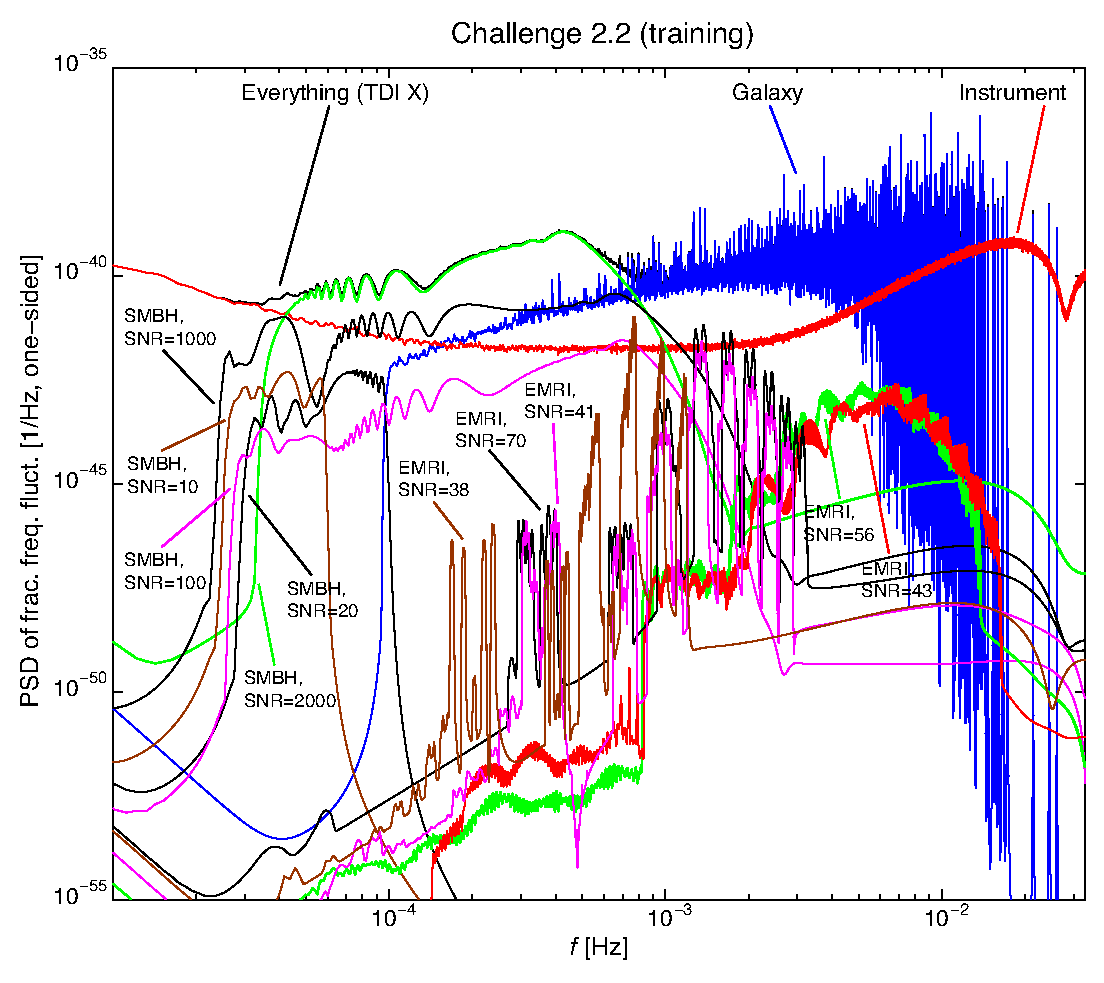
\includegraphics[height=8cm]{challenge-2b}}
\caption{\protect\footnotesize
An example of Challenge 2.2 data set, plotted as the fractional frequency fluctuation spectrum of the full TDI $X$ signal, and separately of instrument noise and of the individual sources (bundling all Galactic binary sources as the ``Galaxy''.)}
\label{f:C2.2}
\end{figure}
%------------------------------    END FIGURE   --------------------------

As in the first round of challenges, we release both blind challenge data sets, where the source parameters are unknown, and training data sets, with GW signals of similar nature to those included in the blind tests, but whose parameters are made public. The training data sets come also in two flavors: ``noisy'' and noise-free, the latter containing exactly the same GW signal(s) as those present in the noisy set. Notice also that, in order to facilitate the development and testing of analysis schemes, Challenge 2.1 and 2.2 training data sets will contain the same realization of the Galaxy, so that the signals from the population of stellar-mass binary systems are identical in the two sets. This will not be the true for the blind sets. 

For each challenge data set the three TDI channels $X$, $Y$ and $Z$ are distributed through the MLDC website~\cite{MLDCweb}. The format in which the MLDC data sets are encoded is implemented using XML (the eXtensible Markup Language), a simple, flexible and widely used text format related to HTML \cite{xml}. Extensive software libraries to handle XML are readily available. The XML implementation of the MLDC file format (known as lisaXML) is based on XSIL (the eXtensible Scientific Interchange Language) \cite{xsil}. A number of dedicated software tools to read and write lisaXML files (for C/C++, Pyhthon, MATLAB and ASCII) were developed by the MLDC Task Force and are available in the LISAtools Subversion archive~\cite{lisatools}. The archive also includes all the software used for the data production pipelines (a detailed ``How To'' for Challenge 2 is also posted on the Task Force wiki \cite{MLDCwiki}), including the waveform generation codes described in the next sections, as well as a variety of other software tools useful to analyze MLDC data sets.

The actual generation of the data sets is the responsibility of one member of the Task Force who does not take part in the challenges. The deadline for submission of results (again through the MLDC website) is June 15th, 2007. The Task Force plans to process the results and provide an initial summary and evauation of this round within about a month of the results being received.

\section{Modeling of LISA: Pseudo-LISA}
\label{s:lisa}

We have developed a set of conventions to describe the LISA orbit and response, which constitute the \emph{pseudo-LISA} adopted in Challenge 1 and 2. The pseudo-LISA orbits are obtained by truncating exact Keplerian orbits for a point mass orbiting the Sun to first order in the eccentricity (see the Appendix of~\cite{lisasimulator}). The two simulators used for the generation of the data sets -- the LISA Simulator \cite{lisasimulator} and Synthetic LISA \cite{synthlisa} -- comply with these assumptions, and adhere to these conventions. In Solar-System Barycentric (SSB) coordinates (with the $x$ axis aligned with the vernal point), we set
%
\begin{eqnarray}
x_n &=& a\cos \alpha + a \, e\left(\sin\alpha\cos\alpha\sin\beta_n
-(1+\sin^2\alpha)\cos\beta_n\right), \nonumber \\
y_n &=& a\sin \alpha + a \, e\left(\sin\alpha\cos\alpha\cos\beta_n
-(1+\cos^2\alpha)\sin\beta_n\right), \\
z_n & = & -\sqrt{3} \, a \, e \cos(\alpha-\beta_n) \, , \nonumber
\end{eqnarray}
%
where $\beta_n = (n-1)\times2\pi/3 + \lambda$ ($n=1, 2, 3$) is the relative orbital phase of the $n$-th spacecraft, $a = 1$ AU is the semi-major axis of the guiding center, $\alpha(t)=2 \pi \, t / (1 \mathrm{year}) + \kappa$ is its orbital phase, and $t$ is time measured at the SSB. In this approximation, the spacecraft form a rigid equilateral triangle with side length $L = 2\sqrt{3} \, a \, e = 5\times 10^6$ km for $e=0.00965$. (In fact, the LISA Simulator and Synthetic LISA implement $e^2$-accurate orbits, but the additional terms make very little difference to the instrument response.) The parameters $\kappa$ and $\lambda$ (\texttt{InitialPosition} and \texttt{InitialRotation} in lisaXML) set the initial location and orientation of the LISA constellation; in Challenge 1, $\kappa=\lambda=0$. This choice places LISA at the vernal point at time $t=0$, with spacecraft 1 directly below the guiding center in the southern ecliptic hemisphere (see~\cite{MLDCdoc} for expressions to convert to other LISA orbit specifications). 
%
\begin{table}
\begin{tabular}{llll}
\hline
{Parameter} &
{Symbol} &
{Standard parameter name} &
{Standard unit} \\
& & (lisaXML descr.) & (lisaXML descr.) \\
\hline
Ecliptic latitude   & $\beta$   & \texttt{EclipticLatitude}  & \texttt{Radian} \\
Ecliptic longitude  & $\lambda$ & \texttt{EclipticLongitude} & \texttt{Radian} \\
Polarization angle  & $\psi$    & \texttt{Polarization}      & \texttt{Radian} \\
Inclination         & $\iota$   & \texttt{Inclination}       & \texttt{Radian} \\
Luminosity distance & $D$       & \texttt{Distance}          & \texttt{Parsec} \\
\hline
\end{tabular}
\caption{Common source parameters. Note that in the initial challenges we do not deal explicitly with the redshifting of sources at cosmological distances; thus, $D$ is a \emph{luminosity} distance, and the masses and frequencies of Tables \ref{tab:bbh} are those measured at the SSB, which are red/blue-shifted by factors $(1+z)^{\pm 1}$ with respect to those measured locally near the sources.\label{tab:common}}
\end{table}

The one-way links between adjacent spacecraft that are necessary to build the LISA response to GWs are either the phase response $\Phi_{ij}$ -- as employed in the LISA Simulator, see Sec.\ II of~\cite{lisasimulator} -- or the fractional frequency response $y^\mathrm{gw}_{slr}$, as used in Synthetic LISA, see Sec.\ II B in~\cite{synthlisa}. The TDI Rosetta Stone~\cite{rosetta} provides details for translations between index notations. The phase and fractional-frequency formalisms are equivalent, and are related by a simple time integration\footnote{\emph{LISA Simulator} produces \emph{equivalent-strain} data, with a nominal length of $L_n = 10^{10}$ m; to convert equivalent strain to fractional frequency one needs to differentiate and multiply by $L_n / c$. The additional factor of $2 \pi$ given in \cite{MLDCLISA06b} for this conversion is incorrect.}.

LISA employs Time-Delay Interferometry (TDI) to suppress the otherwise overwhelming laser phase noise (see~\cite{firstgen,modified,secondgen} and references therein). TDI observables are constructed from time-delayed linear combinations of one-way links, and they represent synthesized interferometers where laser phase fluctuations move in closed paths across the LISA arms. More complicated paths are required to deal with the real-orbit variations of the armlengths, giving rise to the three TDI ``generations''. For the initial MLDCs,  \emph{TDI 1.5} observables \cite{modified,secondgen} are adopted. In particular the data sets are the unequal-arm Michelson observables $X$, $Y$, and $Z$ defined in~\cite{secondgen}. Strictly speaking, TDI 2.0 would be required to cancel laser noise completely in a rotating and flexing LISA array such as the current pseudo-LISA. The difference between TDI 1.5 and 2.0 is negligible for the response to GW signals, but it requires a more complex  numerical treatment of one-way links, adding unnecessary complexity to the analysis. Thus, Challenge data sets 1 and 2 contain TDI 1.5 observables without laser noise.

The model of the LISA instrumental noise $S_\mathrm{in}$ adopted in Challenge 2 is identical to that considered for Challenge 1. It includes contributions from optical noise, assumed white in phase, with one-sided spectral density
\be
S_\mathrm{opt}^{1/2}(f) = 20 \times 10^{-12} \, \mathrm{m}\, \mathrm{Hz}^{-1/2}\,,
\ee
and from acceleration noise (assumed white in acceleration, but increasing as $1/f$ below $10^{-4}$ Hz), with one-sided spectral density 
\be
S_\mathrm{acc}^{1/2}(f) = 3 \times 10^{-15} [1 + (10^{-4}\,{\rm Hz}/f)^2]^{1/2}\, \mathrm{m}\, \mathrm{s}^{-2}\, \mathrm{Hz}^{-1/2}\,;
\ee
the total noise contribution is then simply $S_\mathrm{in} = S_\mathrm{opt}(f) + S_\mathrm{acc}(f)$. As we have mentioned above, the laser phase noise is assumed to be zero. The six optical noises and six acceleration noises (for the two optical benches on each spacecraft) are modelled as independent Gaussian random processes, and are realized in practice with sequences of pseudo-random numbers. Specifically, Synthetic LISA generates independent Gaussian deviates (i.e., white noise) in the time domain, and then filters them digitally to obtain the desired spectral shape; the LISA Simulator generates independent Gaussian deviates in the frequency domain, multiplies them by $S^{1/2}(f)$, and FFTs to the time domain.

\section{Gravitational waveforms}

In this section we describe the conventions adopted to describe the gravitational waveforms and the assumptions made on the signals to construct the data sets. They are identical to those adopted in Challenge 1, but for this challenge we introduce two new ingredients: the model of the Galaxy used to simulate a population of stellar-mass binaries, and the kludge EMRI waveforms.

\subsection{Gravitational wave polarizations}
\label{ss:polarizations}

The sky location of a GW source is described in J2000 \emph{ecliptic coordinates}: latitude $\beta$ and longitude $\lambda$, the latter measured from the vernal point, aligned with the $\hat{x}$ axis in our convention. Gravitational radiation travels along the direction $\hat{k} = -(\cos \beta \cos \lambda, \cos \beta \sin \lambda, \sin \beta)$, with surfaces of constant phase given by $\xi = t - \hat{k} \cdot x$. In the transverse--traceless gauge, the gravitational strain tensor can be decomposed in two polarization states $h_{+}(\xi)$ and $h_{\times}(\xi)$, and is given by
%
\begin{equation}
\label{eq:defpol}
\mathbf{h}(\xi) = h_{+}(\xi) \left[ \hat{u}\otimes \hat{u} - \hat{v}\otimes \hat{v} \right] + h_{\times}(\xi) \left[ \hat{u}\otimes \hat{v} + \hat{v}\otimes \hat{u} \right],
\end{equation}
%
where $\hat{u} = \partial \hat{k} / \partial{\beta}$, $\hat{v} \propto \partial \hat{k} / \partial{\lambda}$. Thus, GWs from any MLDC source are completely specified by $\beta$, $\lambda$, and by the two functions $h_+(\xi)$ and $h_\times(\xi)$ for the source GW polarization amplitudes, measured at the SSB.

The orbital orientation of nonprecessing binaries is described by the inclination $\iota$ (the angle between the line of sight $-\hat{k}$ and the orbital angular momentum of the binary), and by their polarization angle $\psi$: specifically, if $h^S_{+}(\xi)$ and $h^S_\times(\xi)$ are the binary's GW polarizations in the source frame (i.e., defined with respect to the binary's \emph{principal polarization axes} $\hat{p}$ and $\hat{q}$) then 
%
\begin{equation}
h_+(\xi) + i h_\times(\xi) = e^{-2 i \psi} \left[ h^S_+(\xi) + i h^S_\times(\xi) \right],
\end{equation}
%
with $\psi = -\arctan(\hat{v} \cdot \hat{p} / \hat{u} \cdot \hat{p})$.
Together with $\beta$, $\lambda$, and with the luminosity distance $D$, $\iota$ and $\psi$ form a set of common standard parameters, listed in Tab.\ \ref{tab:common} with their standard lisaXML (see \cite{MLDCLISA06b} for a description of the XML files adopted for the MLDCs).

\subsection{Galactic stellar mass binaries}
\label{ss:WD}

In Challenge 2, a Galactic stellar mass binary system of two stars of mass $m_1$ and $m_2$ at distance $D$  is modelled as two point masses in circular orbit with constant period. The source-frame polarization amplitudes are given by
%
\begin{eqnarray}
h^S_+(\xi)  & = & \mathcal{A} \left(1 + \cos^2{\iota}\right) \cos(2\pi f \xi + \phi_0), \\
h^S_\times(\xi) & = & -2 \mathcal{A} (\cos{\iota}) \sin(2\pi f \xi + \phi_0), \nonumber
\end{eqnarray}
%
where the amplitude is derived from the physical parameters of the source as $\mathcal{A} = (2 \mu / D) (\pi M f)^{2/3}$, with $M = m_1 + m_2$ the total mass, and $\mu = m_1 m_2 / M $ the reduced mass; $ \phi_0$ is an arbitrary random initial phase. Notice that $f$ is constant in the SSB, but not in the final LISA data set, because of Doppler shifts induced by the LISA orbital motion.
A Challenge-2 \texttt{GalacticBinary} source is completely determined by the parameters listed in Tables \ref{tab:common} and \ref{tab:galactic}.
%
\begin{table}
\begin{tabular}{llll}
\hline
{Parameter} &
{Symbol} &
{Standard parameter name} &
{Standard unit} \\
& & (lisaXML descr.) & (lisaXML descr.) \\
\hline
Amplitude           & $\mathcal{A}$ & \texttt{Amplitude}    & \texttt{1} (GW strain) \\
Frequency           & $f$           & \texttt{Frequency}    & \texttt{Hertz} \\
Initial GW phase    & $\phi_0$      & \texttt{InitialPhase} & \texttt{Radian} \\
\hline
\end{tabular}
\caption{\texttt{GalacticBinary} source parameters. Note that \texttt{Amplitude} effectively replaces the standard \texttt{Distance} parameter.\label{tab:galactic}}
\end{table}

The data sets 2.1 and 2.2 contain 20 ``verification binaries'', defined as systems whose location and orbital period are exactly known. The remaining 4 parameters are selected randomly. We consider 5 real known systems and then select 15 more from a synthetic model of the Galaxy. The verification binaries have the same sky locations, frequencies and amplitudes as those used in Round 1. In addition to the verification binaries $\sim 26$ million
white dwarf binaries have been included from a population synthesis model. The same set of stellar mass binaries have been used in the training sets for Challenges 2.1 and 2.2 to allow participants to compare the source recovery with and without other signal types present. Different relaizations of the stellar mass binaries are used in each of the blind data sets.

\subsection{Galactic model}
\label{ss:galaxy}

The galactic model is derived from a modern population synthesis code~\cite{gijs}, and contains some 26 million white dwarf binaries.
Rather than re-running the population synthesis code each time a new realization was needed, a single simulation was used and new
versions were created by tweaking the frequencies of the binaries by a random amount of order 3 $\mu$Hz,
and by randomly drawing new values for the inclination, polarization and initial phase. These perturbations are large enough to make the
simulated galaxies distinct from a data analysis perspective, yet small enough to leave the population unaffected from an astrophysical
perspective. 

Since the LISA Simulator and Synthetic LISA take several minutes to process a single source, it is not practical to use them to
generate the response to a full galactic background. Instead a new simulation tool~\cite{cornish_littenberg} was used that
is custom designed for modeling slowly evolving signals. The output of this new tool has been checked against
the LISA Simulator and Synthetic LISA and the results agree to parts in a million. The one place where they differ is
in computational cost, as the dedicated code is able to process the entire galaxy in just a few hours on a single processor.

\subsection{Massive--black-hole binaries}

In these first two rounds of MLDCs, massive-black hole binaries are restricted to having circular orbits and non-spinning black holes. We also consider only the inspiral phase of the whole coalescence process. We model the inspiral at the restricted second post-Newtonian order, following~\cite{Blanchet,DIS}: we first introduce the parameters
\be
\tau =  \frac{\eta}{5M}(t_c - t)
\ee
where $t_c$ is the time at coalescence, and $\eta = \mu/M$. The time evolution of the \emph{orbital} angular frequency $\omega$ and phase $\Phi$ are then given at 2PN order by
\bea
M\omega &=& \frac{1}{8} \tau^{-3/8}\Biggl\{ 1 + \left( \frac{11}{32}\eta + \frac{743}{2688}\right) 
\tau^{-1/4} - \frac{3}{10}\pi\tau^{-3/8} \nonumber \\
& + & \left(\frac{1855099}{14450688} + \frac{371}{2048}\eta^2 
+ \frac{56975}{258048}\eta\right)
\tau^{-1/2}  \Biggr\}
\label{fr}
\eea
and
\bea
\Phi &=& -\frac{1}{32\eta}(M\omega)^{-5/3}\Biggl\{ 1 + \left( \frac{3715}{1008} + \frac{55}{12}\eta\right)
(M\omega)^{2/3} - 10\pi(M\omega)  \nonumber \\
&+&  \left( \frac{15293365}{1016064} + \frac{27145}{1008}\eta + \frac{3085}{144}\eta^2\right)
(M\omega)^{4/3}\Biggr\}\,,
\label{eq:Phi}
\eea
respectively. The phase of the polarization waveforms, see below, is then computed according to $\Phi(t) - \Phi(t = 0) + \Phi_0$, where $\Phi_0$ is an arbitrary initial orbital phase.

In the source reference frame, the polarization waveforms are given by:
%
\begin{eqnarray}
h^S_{+}(\xi) &=& \frac{2\mu}{D}[M\omega(\xi)]^{2/3}(1+\cos^2 \iota)\cos [2\Phi(\xi)], \\
h^S_{\times}(\xi) &=& -\frac{2\mu}{D}[M\omega(\xi)]^{2/3}(2 \cos \iota) \sin [2\Phi(\xi)]. 
\end{eqnarray}
%
In order to avoid numerical artifacts at the end of the inspiral (i.e., the last stable orbit), we taper the signal according to:
%
\begin{equation}
w(t) = \frac{1}{2}\,\left( 1 + \tanh\left[A (M/R - M/R_\mathrm{taper})\right] \right)\,,
\end{equation}
%
where $R$ is approximated with Kepler's law ($R = M^{1/3} \omega^{-2/3}$), and
where the dimensionless coefficient $A = 150$ was determined empirically to produce smooth damping; $R_\mathrm{taper}$ is set to $7\, M$.

The lisaXML standard parameters for Challenge-2 \texttt{BlackHoleBinary} sources are listed in Tables \ref{tab:common} and \ref{tab:bbh}.
%
\begin{table}
\begin{tabular}{llll}
\hline
{Parameter} &
{Symbol} &
{Standard parameter name} &
{Standard unit} \\
& & (lisaXML descr.) & (lisaXML descr.) \\
\hline
Mass of first BH    & $m_1$  & \texttt{Mass1}           & \texttt{SolarMass} \\
Mass of second BH   & $m_2$  & \texttt{Mass2}           & \texttt{SolarMass} \\
Time of coalescence & $t_c$  & \texttt{CoalescenceTime} & \texttt{Second} \\
Angular orbital phase & $\Phi_0$ & \texttt{InitialAngularOrbitalPhase} & \texttt{Radian} \\
\multicolumn{1}{r}{at time $t = 0$} & & & \\
Tapering radius & $R$    & \texttt{TaperApplied}    & \texttt{TotalMass} \\ 
\hline
\end{tabular}
\caption{\texttt{BlackHoleBinary} source parameters.\label{tab:bbh}}
\end{table}

\subsection{Extreme--Mass-Ratio Inspirals}

Extreme--Mass-Ratio Inspirals -- compact objects (CO) orbiting a MBH -- constitute the new source class included in the second round of MLDCs. The EMRI waveforms adopted are the Barack--Cutler ``analytic kludge'' waveforms \cite{BC}, where orbits are instantaneously approximated as Newtonian ellipses and gravitational radiation is given by the corresponding Peters--Matthews formula \cite{pm}, but perihelion direction, orbital plane, semi-major axis, and eccentricity evolve according to post-Newtonian equations. While these waveforms are not particularly accurate in the highly relativistic regime of interest for real EMRI searches, they do exhibit the main qualitative features of the true waveforms, and they are considerably simpler to generate.  They are therefore ideal to develop and test search strategies. It is expected that any search strategy that works for them could be modified fairly easily to deal with the true general-relativistic waveforms, once these become available.

In general relativity, the full two-body system is described by 17 parameters. Here we assume that the spin of the CO is negligible with respect to the MBH's spin and can therefore be ignored: the signal is then described by 14 parameters, which we now describe. Let us consider a CO of mass $\mu$ $(\ll M)$ orbiting a MBH of mass $M$ on an orbit with semi-major axis $a$, eccentricity $e$ and \emph{orbital} frequency $\nu$. At the Newtonian order,  $\nu = (2\pi M)^{-1} (M/a)^{3/2}$, and the \emph{orbital} mean anomaly $\Phi$ (i.e., the average orbital phase with respect to the direction of pericenter) is $\Phi(t) = 2\pi\nu (t-t_0) +\Phi_0$, where  $\Phi_0$ is the mean anomaly at $t_0$. The spin $\vec S$ of the MBH is parametrized by its magnitude $S$ (so that $0 \le S/M^2 \le 1$) and by the two polar angles $\theta_K,\phi_K$ in the SSB (here ``K'' stands for Kerr). $\vec L(t)$ represents the time-varying orbital angular momentum: its direction is parametrized by the \emph{constant} angle $\lambda$ (not to be confused with the ecliptic longitude, defined in Sec~\ref{ss:polarizations}) between $\vec L$ and $\vec S$%
\footnote{In reality, radiation reaction will impose a small time variation in $\lambda$; however, this variation is known to be very small, see~\cite{scott1}, and is neglected here.}, and by an azimuthal angle $\alpha(t)$ that describes the direction of $\hat L$ around $\hat S$. The angle $\tilde\gamma(t)$ is the (intrinsic) direction of pericenter, measured with respect to $\vec L\times\vec S$. Fixing the initial time $t_0$ (as measured in the SSB), $\nu_0$, $e_0$, $\tilde\gamma_0$, and $\Phi_0$ describe, respectively, the eccentricity, the direction of the pericenter within the orbital plane, and the mean anomaly at $t_0$. More specifically, $\tilde\gamma_0$ is the angle in the plane of the orbit from $\hat L \times \hat S$ to pericenter, and $\Phi_0$ is the mean anomaly with respect to pericenter passage. We refer the reader to Figure 1 of Ref.~\cite{BC} for a graphic representation of the system.

It is useful to describe the gravitational wave tensor in a time-varying frame defined with respect to the unit vector ${\hat n} = -{\hat k}$ pointing from the origin of the SSB to the source and ${ \hat L}(t)$. Defining the unit vectors 
${ \hat p}$ and ${ \hat q}$ by
\begin{eqnarray} \label{pq}
{ \hat p} &\equiv& ({ \hat n}\times { \hat L})/
                    |{ \hat n}\times { \hat L}|, \nonumber\\
{ \hat q} &\equiv& { \hat p} \times { \hat n}\,,
\end{eqnarray}
the general GW strain field at the SSB can then be written as
%
\begin{equation}
\label{eq:hab}
\mathbf{h}(\xi) = h_{+}(\xi) \left[ \hat{p}\otimes \hat{p} - \hat{q}\otimes \hat{q} \right] + h_{\times}(\xi) \left[ \hat{p}\otimes \hat{q} + \hat{q}\otimes \hat{p} \right]\,.
\end{equation}
%
Notice that the two polarization basis tensors $[ \hat{p}\otimes \hat{p} - \hat{q}\otimes \hat{q}]$  and $[ \hat{p}\otimes \hat{q} + \hat{q}\otimes \hat{p}]$ are function of time. 
One can decompose Eq.\ (\ref{eq:hab}) into $n$-harmonic contributions at integer multiples of the orbital frequency,
\be
h_{+}\equiv \sum_n A^{+}_n, \quad h_{\times}\equiv \sum_n A^{\times}_n,
\label{harmonics}
\ee
where the $A^{+,\times}_n$ are
\begin{eqnarray} \label{A}
A^{+}_n &=&-[1+({ \hat L}\cdot{ \hat n})^2]\left[
a_n\cos(2\gamma)-b_n\sin(2\gamma)\right]
+[1-({ \hat L}\cdot{ \hat n})^2]c_n, \nonumber\\
A^{\times}_n&=& 2({ \hat L}\cdot{ \hat n})\left[
b_n \cos(2\gamma)+a_n \sin(2\gamma)\right]\,.
\end{eqnarray}
The harmonics $A^{+,\times}_n$ are expressed as a function of the coefficients
\begin{eqnarray} \label{abc}
a_n &=& - n{\cal A}\bigl[J_{n-2}(ne)-2eJ_{n-1}(ne) \nonumber \\
       && +(2/n)J_n(ne) +2eJ_{n+1}(ne)-J_{n+2}(ne)\bigr]\cos[n\Phi(t)],
\nonumber\\
b_n &=& - n{\cal A}(1-e^2)^{1/2}\bigl[J_{n-2}(ne)-2J_{n}(ne)
+J_{n+2}(ne)\bigr]\sin[n \Phi(t)],
\nonumber\\
c_n &=& 2{\cal A}J_n(ne)\cos[n\Phi(t)]\,.
\end{eqnarray}
Here the $J_n$ are Bessel functions of the first kind, and $\gamma$ is an azimuthal angle measuring the direction of pericenter with respect to $\hat x \equiv [-\hat n + \hat L (\hat L\cdot \hat n)]/[1-(\hat L\cdot \hat n)^2]^{1/2}$.
The angle $\gamma$ is related to $\tilde \gamma$ by
\be
\label{beta}
\gamma = \tilde\gamma + \beta,
\ee
where $\beta$ is the angle from $\hat x \propto [\hat L(\hat L \cdot \hat n) \hat n] $ to $(\hat L \times \hat S)$, as given by
\begin{eqnarray}\label{sinbeta}
\sin\beta &=& \frac{\cos\lambda\, \hat L\cdot\hat n -\hat S\cdot \hat n }
{\sin\lambda\bigl[1 - (\hat L\cdot\hat n)^2\bigr]^{1/2}}, \nonumber \\
\cos\beta &=& \frac{\hat n \cdot (\hat S \times \hat L)}
{\sin\lambda\bigl[1 - (\hat L\cdot\hat n)^2\bigr]^{1/2} }.
\end{eqnarray}
%
The overall amplitude is given by
\begin{equation} \label{calA}
{\cal A}\equiv (2\pi \nu M)^{2/3}\frac{\mu}{D}\,.
\end{equation}
In practice, we truncate the sums in Eq.~(\ref{harmonics}) at $n=4$ if $e < 0.136$, otherwise at $n = 30\times e$.

The angular momentum direction vector $\hat L$ is not constant, since $\hat L$ precesses about the MBH's spin
direction $\hat S$.  Let $\theta_L(t),\phi_L(t)$ be the angles specifying the instantaneous direction of $\hat L$, and let $\hat z$ be a unit vector normal to the ecliptic. One then obtains
\be \label{alpha}
\hat L = \hat S \, \cos\lambda +
\frac{\hat z - \hat S \cos\theta_K}{\sin\theta_K} \sin\lambda \cos\alpha
+ \frac{\hat S \times \hat z}{\sin\theta_K}  \, \sin\lambda \sin\alpha\,,
\ee
\noindent
and the angles $\theta_L(t),\phi_L(t)$ are given in terms of $\theta_K$, $\phi_K$,$\lambda$, $\alpha(t)$ by
\begin{eqnarray}\label{relations3}
\cos\theta_L(t) &=& \cos\theta_K \cos\lambda
    +\sin\theta_K\sin\lambda\cos\alpha(t), \nonumber\\
\sin\theta_L(t)\cos\phi_L(t) &=&
\sin\theta_K\cos\phi_K\cos\lambda \nonumber \\
& & -\cos\phi_K\cos\theta_K\sin\lambda\cos\alpha(t)
+\sin\phi_K\sin\lambda\sin\alpha(t),  \nonumber\\
\sin\theta_L(t)\sin\phi_L(t) &=&
\sin\theta_K\sin\phi_K\cos\lambda \nonumber \\
& & -\sin\phi_K\cos\theta_K\sin\lambda\cos\alpha(t) \nonumber \\
& & -\cos\phi_K\sin\lambda\sin\alpha(t).
\end{eqnarray}
%
To work with these expressions, the following relations are useful:
\be
\label{SdotN}
{ \hat S}\cdot{ \hat n} = \cos\theta_S \cos\theta_K
+ \sin\theta_S \sin\theta_K \cos(\phi_S-\phi_K),
\ee
\bea\label{ScrossLdotN}
\hat n \cdot (\hat S \times \hat L) & = &
\sin\theta_S \sin(\phi_K-\phi_S)\sin\lambda \cos\alpha \nonumber \\
& &+ \frac{\hat S\cdot\hat n \cos\theta_K -\cos\theta_S}{\sin\theta_K}
\, \sin\lambda \sin\alpha,
\eea
and
\bea
\label{LdotN}
{ \hat L}\cdot{ \hat n} & = & { \hat S}\cdot{ \hat n}\cos\lambda
+ \frac{\cos\theta_S - \hat S\cdot\hat n \cos\theta_K}{\sin\theta_K}
\, \sin\lambda \cos\alpha \nonumber \\
& & + \frac{(\hat S \times \bar z)\cdot \hat n}
{\sin\theta_K}  \, \sin\lambda \sin\alpha\,, \nonumber \\
& = & \cos\theta_S \cos\theta_L +
\sin\theta_S \sin\theta_L \cos(\phi_S-\phi_L).
\eea
Note that the time-variation of ${ \hat S}\cdot{ \hat n}$ is very small in the extreme mass-ratio case considered here, and in our kludged approximation we approximate $\hat S$ -- and hence ${\hat S}\cdot{\hat n}$ -- as strictly constant.

The evolution of $\Phi(t)$, $\nu(t)$, $\tilde\gamma(t)$, $e(t)$, and $\alpha(t)$ is given by the following PN formulas:
\begin{eqnarray}
\frac{d\Phi}{dt} &=& 2\pi\nu, \label{Phidot} \\
\frac{d\nu}{dt} &=&
\frac{96}{10\pi}(\mu/M^3)(2\pi M\nu)^{11/3}(1-e^2)^{-9/2}
\Bigl\{
\left[1+(73/24)e^2+(37/96)e^4\right](1-e^2) \nonumber \\
&&+ (2\pi M\nu)^{2/3}\left[(1273/336)-(2561/224)e^2-(3885/128)e^4
-(13147/5376)e^6 \right] \nonumber \\
&&- (2\pi M\nu)(S/M^2)\cos\lambda (1-e^2)^{-1/2}[(73/12)
+ (1211/24)e^2 \nonumber \\
&&+(3143/96)e^4 +(65/64)e^6]
\Bigr\}, \label{nudot} \\
%
\frac{d\tilde\gamma}{dt} &=& 6\pi\nu(2\pi\nu M)^{2/3} (1-e^2)^{-1}
\left[1+(2\pi\nu M)^{2/3} (1-e^2)^{-1}(26-15e^2)/4\right] \nonumber \\
&&-12\pi\nu\cos\lambda (S/M^2) (2\pi M\nu)(1-e^2)^{-3/2},
\label{Gamdot} \\
%
\frac{de}{dt}  &=& -\frac{e}{15}(\mu/M^2) (1-e^2)^{-7/2} (2\pi M\nu)^{8/3}
\bigl[(304+121e^2)(1-e^2)\bigl(1 + 12 (2\pi M\nu)^{2/3}\bigr) \, \nonumber \\
&&- \frac{1}{56}(2\pi M\nu)^{2/3}\bigl( (8)(16705) + (12)(9082)e^2 - 25211e^4 \bigr)\bigr]\,
\nonumber \\
&&+ e (\mu/M^2)(S/M^2)\cos\lambda\,(2\pi M\nu)^{11/3}(1-e^2)^{-4}
\, \bigl[(1364/5) + (5032/15)e^2 \nonumber \\ && + (263/10)e^4\bigr] ,
\label{edot} \\
%
\frac{d\alpha}{dt} &=& 4\pi\nu (S/M^2) (2\pi M\nu)(1-e^2)^{-3/2}.
\label{alphadot}
\end{eqnarray}
%
For a point particle in Schwarzschild, the plunge occurs at
$a_{\rm min} = M (6 + 2e)(1-e^2)^{-1}$ \cite{ckp},
so we set
\be\label{numax}
\nu_{\rm max} = (2\pi M)^{-1}[(1-e^2)/(6 + 2e)]^{3/2} \, ,
\ee
and we shut-off the waveform when $\nu$ reaches this $\nu_{\rm max}$.

Equation (\ref{eq:hab}) expresses the waveform in terms of time-varying polarization tensors, but to generate the LISA responses it is necessary to re-express it in terms of fixed polarization tensors. This is achieved through a rotation by the polarization angle
\begin{equation}\label{psiSL}
\psi = \mathrm{arctan}\left(\frac{\sin\theta_L \sin(\phi_S-\phi_L)}{\cos \theta_S \sin \theta_L \cos(\phi_S - \phi_L) - \cos\theta_L \sin\theta_S}\right) - \psi_0\,.
\end{equation}

The algorithm for constructing the MLDC EMRI waveforms works as follows. One fixes a fiducial frequency $\nu_0$ at $t_0 = 0$ and chooses the waveform parameters $\mu,\, M,\,S/M^2,\,e_0,\,\tilde\gamma_0,\,\Phi_0,\,\cos\theta_S,\,\phi_S,\,\cos\lambda,\,\alpha_0,\cos\theta_K,\,\phi_K,\psi_0,D$. One then (i) solves the ODEs (\ref{Phidot})--(\ref{alphadot}) for $\Phi(t)$, $\nu(t)$, $\tilde\gamma(t)$, $e(t)$, $\alpha(t)$; (ii) uses $e(t)$ and $\nu(t)$ to calculate $a_n(t), b_n(t), c_n(t)$ in Eqs.~(\ref{abc}); (iii) calculates $\theta_L(t),\phi_L(t)$ using Eqs.~(\ref{relations3}), and then obtains $\gamma(t)$ from $\tilde\gamma(t)$ using Eqs.~(\ref{beta})--(\ref{sinbeta}); (iv) computes the amplitude coefficients $A_n^{+,\times}$  using Eqs.~(\ref{A}) and (\ref{LdotN}); (v) calculates $\psi$ using Eq.~(\ref{psiSL}); (vi) finally,  $h_{+,\times}(t)$ are computed using the following equations
\begin{eqnarray}\label{final}
h_+(t) = A^+(t) cos(2\psi_0 - 2\psi_{SL}(t) ) + A^{\times}(t) sin(2\psi_0 - 2\psi_{SL}(t) ) \nonumber \\
h_{\times}(t) = A^{\times}(t) cos(2\psi_0 - 2\psi_{SL}(t) ) - A^+(t) sin(2\psi_0 - 2\psi_{SL}(t) )
\end{eqnarray}


The lisaXML standard parameters for Challenge-2 \texttt{ExtremeMassRatioInspiral} sources are listed in Tables \ref{tab:common} and \ref{tab:emri}.
%
\begin{table}
\begin{tabular}{llll}
\hline
{Parameter} &
{Symbol} &
{Standard parameter name} &
{Standard unit} \\
& & (lisaXML descr.) & (lisaXML descr.) \\
\hline
Mass of central BH     & $M$      & \texttt{MassOfSMBH}           & \texttt{SolarMass} \\
Mass of compact object & $\mu$  & \texttt{MassOfCompactObject}  & \texttt{SolarMass} \\
Central-BH spin        & $|S|/M^2$  & \texttt{CoalescenceTime}      & \texttt{Second} \\
Central-BH spin orientation & $\theta_K, \phi_K$ & \texttt{PolarAngleOfSpin}, & \texttt{Radian} \\
 \multicolumn{1}{r}{w.r.t. SSB frame}  &                         & \texttt{AzimuthalAngleOfSpin} & \\ \hline
& & \texttt{InitialAzimuthal}\ldots & \\                   
Radial orbital freq.\ at $t = 0$ & $\nu_0$ & \multicolumn{1}{r}{\ldots\texttt{OrbitalFrequency}} & \texttt{Hertz} \\
Orbital mean anomaly at $t = 0$ & $\Phi_0$ & \multicolumn{1}{r}{\ldots\texttt{OrbitalPhase}} & \texttt{Radian} \\ \hline
Eccentricity at $t = 0$ & $e_0$ & \texttt{InitialEccentricity} & \texttt{1} \\
Direction of pericenter at $t = 0$ & $\tilde{\gamma}_0$ & \texttt{InitialTildeGamma} & \texttt{Radian} \\
Direction of orbital angular & $\alpha_0$ & \texttt{InitialAlphaAngle} & \texttt{Radian} \\
\multicolumn{1}{r}{momentum w.r.t. $S$ at $t = 0$} & & & \\
Opening angle & $\lambda$ & \texttt{LambdaAngle} & \texttt{Radian} \\ 
\hline
\end{tabular}
\caption{\texttt{ExtremeMassRatioInspiral} source parameters. Note that EMRIs do not use the nonprecessing-binary inclination $\iota$, and be aware of the collision between the symbols for the EMRI compact-object mass ($\mu$) and opening angle ($\lambda$), the binary reduced mass (again $\mu$), and the ecliptic longitude (again $\lambda$). Note that $\nu$ is called ``Azimuthal orbital frequency'' in the XML file and it is referred to as a radial orbital frequency in \cite{BC}.
If we reduce the equations to non-spinning MBH and circular orbits, then 
the orbital frequency corresponds to $\nu + \dot{\tilde{\gamma}}/{2\pi}$.
\label{tab:emri}}
\end{table}

\section{Conclusions}

The Mock Data Challenges (MLDCs) are aimed at stimulating the development of LISA data analysis capabilities, and demonstrating the technical readiness to tackle LISA data sets. The first round of MLDCs has just been completed and the second round data sets have been released. The latter provide a fairly realistic testbed of analysis techniques to attack the new analysis challenges posed by the mission, in particular the observation of extreme-mass-ratio inspirals and aspects of "global data analysis". 


\section*{Acknowledgments}
M.V.'s work was supported by the LISA Mission Science Office and by the Human Resources Development Fund at the Jet Propulsion Laboratory, California Institute of Technology, where it was performed under contract with the National Aeronautics and Space Administration.


\section*{References}
\begin{thebibliography}{10}
\bibitem{ScienceCase} LISA Mission Science Office, ``LISA: probing the universe with gravitational waves'', v. 1.0 (2007), available at \url{www.lisascience.org/resources}.
\bibitem{lisappa} LISA Study Team, ``LISA: Laser Interferometer Space Antenna for the detection and observation of gravitational waves'', Pre-Phase A Report, 2nd ed. (Max Planck Institut f\"ur Quantenoptik, Garching, Germany, 1998).
%
\bibitem{CT2002} Cutler C and Thorne K S, in \emph{General Relativity and Gravitation}, N. T. Bishop and D. M. Sunil, eds. (World Scientific, Singapore, 2002), p. 72.
\bibitem{MLDCweb} Mock LISA Data Challenge Homepage, \url{astrogravs.nasa.gov/docs/mldc}.
\bibitem{MLDC1-gwdaw} Arnaud K A, {\it et al.} 2007 (gr-qc/0701139).
\bibitem{xml} World Wide Web Consortium (W3C), ``eXtensible Markup Language (XML) activity and information'', \texttt{www.w3.org/XML}.
\bibitem{xsil} Caltech Center for Advanced Computing Research, ``XSIL: Extensible Scientific Interchange Language'', \texttt{www.cacr.caltech.edu/SDA/xsil}.
\bibitem{MLDCLISA06a} Arnaud K A, {\it et al.} 2006 {\it AIP Conf. Proc.} {\bf 873} 619 (\url{gr-qc/0609105}).
\bibitem{MLDCLISA06b} Arnaud K A, {\it et al.} 2006 {\it AIP Conf. Proc.} {\bf 873} 625 (long version with lisaXML description: \url{gr-qc/0609106}).
\bibitem{MLDCwiki} Mock LISA Data Challenge Task Force wiki, \url{www.tapir.caltech.edu/dokuwiki/listwg1b:home}.
\bibitem{MLDCdoc} Mock LISA Data Challenge Task Force, ``Document for Challenge 1'', \url{svn.sourceforge.net/viewvc/lisatools/Docs/challenge1.pdf}.
\bibitem{lisasimulator} Cornish N J and Rubbo L J, \emph{Phys. Rev. D} \textbf{67}, 022001 (2003); erratum, \emph{ibid.}, 029905 (2003); LISA Simulator website, \texttt{www.physics.montana.edu/lisa}; the canonical MLDC releases of Synthetic LISA are also available from the SourceForge MLDC site \cite{lisatools}.
\bibitem{synthlisa} Vallisneri M, \emph{Phys. Rev. D} \textbf{71}, 022001 (2005); Synthetic LISA website, \texttt{www.vallis.org/syntheticlisa}; the canonical MLDC releases of Synthetic LISA are also available from the SourceForge MLDC site \cite{lisatools}.
\bibitem{rosetta} M. Vallisneri, the \emph{TDI Rosetta Stone} v. 1/5/2005, \texttt{www.vallis.org/tdi}.
\bibitem{firstgen} (TDI 1.0) Armstrong J W, Estabrook F B, and Tinto M,
\emph{Astrophys. J.} \textbf{527}, 814 (1999); Estabrook F B, Tinto M, and Armstrong J W, \emph{Phys. Rev. D} \textbf{62}, 042002 (2000).
\bibitem{modified} (TDI 1.5) Cornish N J and Hellings R W, \emph{Clas. Quant. Grav.} \textbf{20}, 4851 (2003).
\bibitem{secondgen} (TDI 2.0) Shaddock D A, Tinto M, Estabrook F B, and Armstrong J W, \emph{Phys. Rev. D} \textbf{68}, 061303(R) (2003); Tinto M, Estabrook F B, and Armstrong J W, \emph{Phys. Rev. D} \textbf{69}, 082001 (2004).
\bibitem{lisatools} LISAtools SourceForge Project, \texttt{sourceforge.net/projects/lisatools}; the LISAtools Subversion code archive is accessible from 
\url{sourceforge.net/svn/?group_id=161442}.
\bibitem{Blanchet} Blanchet L, Faye G, Iyer B R, Joguet B, \emph{Phys. Rev. D} \textbf{65}, 061501 (2002); \emph{erratum}, \textbf{71}, 129902(E) (2005).
\bibitem{DIS} Damour T, Iyer B R, Sathyaprakash B S, \emph{Phys. Rev. D} \textbf{63}, 044023 (2001).
\bibitem{gijs} Nelemans G, Yungelson L R\& Portegies Zwart S F, A\&A {\bf 375}, 890 (2001).
\bibitem{cornish_littenberg} Cornish N J\& Littenberg T, {\em in preparation}.
\bibitem{BC} Barack L and Cutler C, \emph{Phys. Rev. D} {\bf 69}, 082005 (2004).
\bibitem{pm} Peters P C and Mathews J, \emph{Phys. Rev. D} {\bf 131}, 435 (1963);
 Peters P C, \emph{Phys. Rev. D} {\bf 136}, B1224 (1964).
\bibitem{scott1} Hughes S A, \emph{Phys. Rev. D} {\bf 61}, 084004 (2000).
\bibitem{ckp} Cutler C, Kennefick D, and Poisson E, \emph{Phys. Rev. D} {\bf 50}, 3816 (1994).


\end{thebibliography}

\end{document}
